%
% sa.tex - exemplo de artigo para o Seminário de Andamento
% $Id: sa.tex,v 1.1.1.1 2005/01/18 23:54:44 avila Exp $
%
% UFRGS TeX Users Group
% Institute of Informatics --- UFRGS
% Porto Alegre, Brazil
% http://www.inf.ufrgs.br/utug
% Discussion list: utug-l@inf.ufrgs.br
%
% Copyright (C) 2001 UFRGS TeX Users Group
% This is free software, distributed under the GNU GPL; please take
% a look in `iiufrgs.cls' to see complete information on using, copying
% and redistributing these files
%
\documentclass{sa}
\usepackage[latin1]{inputenc}
\usepackage{graphicx}

\title{Formato dos artigos para a Semana Acadêmica do PPGC da UFRGS}
\author{%
\mbox{UFRGS} {\TeX} Users Group\\
Leslie Lamport (orientador)\\
Donald E. Knuth (co-orientador)\\
utug-l@inf.ufrgs.br
}

\begin{document}
\maketitle

%---------------------------------------------------------------------------
\begin{abstract}
Este documento apresenta as instruções para o formato dos artigos a serem 
incluídos nos Anais da Semana Acadêmica do PPGC da UFRGS, que reúne os 
Seminários de Andamento das Dissertações de Mestrado em elaboração no curso. 
Este Resumo não deve conter menos do que 6~(seis) e mais do que 8~(oito) 
linhas. Ele deve introduzir claramente qual é o tema principal da Dissertação 
de Mestrado e as principais vantagens ou características da metodologia ou 
sistema sendo desenvolvido. A palavra Resumo deve ser escrita em negrito. 
O texto do Resumo deve ser escrito em itálico.
\end{abstract}
%---------------------------------------------------------------------------
\section{INTRODUÇÃO}
\label{sec:intro}
O artigo deve ser escrito em Português e dividido em seções numeradas
seqüencialmente. Sub-seções não podem ser utilizadas. A
Seção~\ref{sec:intro} deve se chamar necessariamente Introdução e deve
situar o tema da dissertação dentro de uma sub-área da Computação,
assim como apresentar a motivação para o desenvolvimento do
trabalho. As páginas não devem ser numeradas.

O artigo deve ocupar 4~páginas, nem mais, nem menos. Ele deve ter a
estrutura e o nível esperado de um artigo publicado numa conferência
ou revista, ou seja, espera-se que ele introduza um problema,
apresente a motivação para o desenvolvimento de uma solução, situe a
abordagem proposta para esta solução dentro do estado-da-arte, e
descreva esta solução com o grau de detalhamento que for possível,
tendo em vista o atual estágio de desenvolvimento da dissertação.
%---------------------------------------------------------------------------
\section{FONTES, MARGENS E ESTILOS}
O artigo deve ser escrito com fonte Times, tamanho~11. O texto deve utilizar 
espaçamento 1~(um) entre as linhas. Os parágrafos não devem ter recuo na 
primeira linha e devem ser separados entre si por uma linha em branco. O 
texto deve ser ajustado à direita. O artigo deve ser impresso em papel~A4, 
com margem superior de 2,5~cm, margem inferior de 2,0~cm e margens laterais 
de 2,0~cm.

O título do trabalho deve ser escrito em tamanho~14, em negrito, e deve 
estar centrado na página, sendo deixada uma linha em branco acima do mesmo. 
Abaixo do título, separada deste por duas linhas, deve constar a identificação 
do mestrando e de seu orientador, utilizando tamanho~11, em negrito, também 
centrada na página. A expressão ``(orientador)'' deve constar explicitamente 
ao lado do nome do orientador. Se o trabalho tiver um co-orientador, a 
referência a este deve ser incluída. Os títulos das seções devem ser escritos 
em letras maiúsculas, usando negrito. O título de uma nova seção deve ser 
separado por duas linhas do final da seção anterior. Evite o uso de negrito 
no meio de texto para enfatizar alguma palavra ou expressão. 
Dê preferência ao uso do \emph{itálico}. Não utilize notas de rodapé.
%---------------------------------------------------------------------------
\section{FIGURAS E TABELAS}
Figuras e tabelas devem estar centradas na página. Os títulos (\emph{captions}) 
das mesmas também devem estar centrados, e devem ser escritos com o mesmo 
fonte do restante do texto. Figuras devem ser numeradas seqüencialmente, de 
1 a~N, em numeração única ao longo de todo o texto. A Figura~\ref{fig} permite 
verificar o estilo desejado para as figuras do artigo (exceto pelo idioma, 
que deveria ser o mesmo usado no restante do texto). Tabelas também devem 
seguir uma numeração única própria, de 1 a~N\@. Detalhes pequenos demais nas 
figuras devem ser evitados em função da legibilidade ou visibilidade.

\begin{figure}
	\centerline{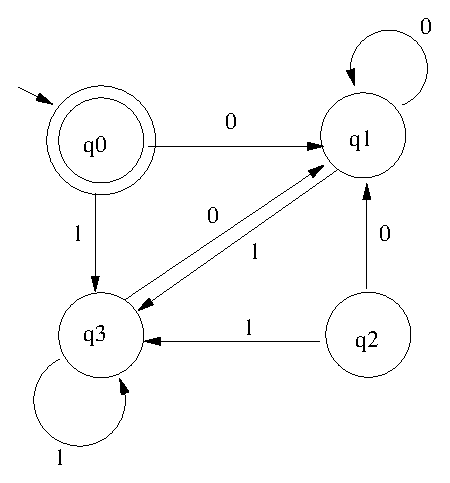
\includegraphics[width=4cm]{fig.eps}}
	\caption{Exemplo de utilização de figura no texto.}
	\label{fig}
\end{figure}

%---------------------------------------------------------------------------
\section{REFERÊNCIAS BIBLIOGRÁFICAS}
Referências bibliográficas devem aparecer no texto entre colchetes~\cite{chu}, e 
devem ser identificadas por uma numeração seqüencial~\cite{wagner}, conforme a 
ordem em que aparecerem ao longo do texto. No final do artigo, as referências 
devem ser listadas segundo a numeração e devem seguir os formatos 
exemplificados neste documento~\cite{chu}, que ilustram referências a 
relatórios de pesquisa, livros, artigos em conferências e artigos em revistas. 
Não referencie literatura em excesso! Limite-se às referências mais importantes.
%---------------------------------------------------------------------------
\section{CONCLUSÕES}
A última seção do artigo deve chamar-se necessariamente Conclusões e deve 
apresentar um resumo das principais contribuições do trabalho e uma síntese do 
trabalho previsto para a próxima etapa (curto prazo).

Muito bem. Você já sabe como formatar seu artigo para o Seminário de Andamento. Agora faça o download da classe \LaTeX\ \texttt{sa.cls}~\cite{lamport} e esqueça todos os detalhes de formatação recém apresentados.
%---------------------------------------------------------------------------
\section*{AGRADECIMENTOS}
Caso o mestrado esteja sendo apoiado por bolsa de estudos de alguma agência 
de fomento ou tenha apoio de alguma universidade/empresa, um agradecimento 
deve ser incluído. Agradecimentos a pessoas que estejam colaborando de 
forma relevante para o trabalho também podem ser incluídos.
%---------------------------------------------------------------------------
\begin{thebibliography}{10}
\bibitem{chu}
Y.~Chu. \underline{Introduction to Computer Organization}. Englewood Cliffs, 
Prentice Hall, 1970.

\bibitem{wagner} F.~Wagner, I.~Jansch-Pôrto, T.S.~Weber e R.F.~Weber. 
Uma proposta de currículo em arquitetura de computadores. In:
\underline{Workshop de Educação em Informática, II}. Caxambu, Agosto 1994. 
Anais. SBC/UFMG, 1994, pp 41-57.

\bibitem{lamport} L.~Lamport. \underline{\LaTeX}: a Document Preparation System. Addison-Wesley, 1994. 2.ed.
\end{thebibliography}
\end{document}
